\chapter{Introduction}

\section{Introduction}
\label{sec:intro}

% Queries in MDE: scalability challenge
Nowadays, model-driven software engineering (MDE) plays an important role in the development processes of critical embedded systems. Advanced modeling tools provide support for a wide range of development tasks such as requirements and traceability management, system modeling, early design validation, automated code generation, model-based testing and other validation and verification tasks. 
With the dramatic increase in complexity that is also affecting critical embedded systems in recent years, modeling toolchains are facing scalability challenges as the size of design models constantly increases, and automated tool features become more sophisticated.

% The role/importance  of expressive and incremental queries in MDE
Many scalability issues can be addressed by improving query performance. \emph{Incremental evaluation} of model queries aims to reduce query response time by limiting the impact of model modifications to query result calculation. Such algorithms work by either (i) building a cache of interim query results and keeping it up-to-date as models change (e.g.\ \incquery{}~\cite{models10}) or (ii) applying impact analysis techniques and re-evaluating queries only in contexts that are affected by a change (e.g.\ the Eclipse OCL Impact Analyzer~\cite{OCLIA}). This technique has been proven to improve performance dramatically in several scenarios (e.g.\ on-the-fly well-formedness validation or model synchronization), at the cost of increasing memory consumption. Unfortunately, this overhead is combined with the increase in model sizes due to in-memory representation (found in state-of-the-art frameworks such as EMF~\cite{EMF}). Since single-computer heaps cannot grow arbitrarily (as response times degrade drastically due to garbage collection problems), memory consumption is the most significant scalability limitation.% of the single workstation architecture.


% Scalability for databases and linked data
% graph databases, RDF/SPARQL
% at the cost of expressive ad-hoc queries

An alternative approach to tackling MDE scalability issues is to make use of advances in persistence technology. As the majority of model-based tools uses a graph-oriented data model, recent results of the NoSQL and Linked Data movement~\cite{neo4j,openvirtuoso,sesame} are straightforward candidates for adaptation to MDE purposes. Unfortunately, this idea poses difficult conceptual and technological challenges: (i) property graph databases lack strong metamodeling support and their query features are simplistic compared to MDE needs, and (ii) the underlying data representation format of semantic databases (RDF~\cite{website:rdf_standard}) has crucial conceptual and technological differences to traditional metamodeling languages such as Ecore~\cite{EMF}. Additionally, while there are initial efforts to overcome the mapping issues between the MDE and Linked Data worlds~\cite{hillairet2008bridging}, even the most sophisticated NoSQL storage technologies lack efficient and mature support for executing expressive queries incrementally.

% Goals: scale up to large models, yet maintain scalability for expressive and incremental queries
% proposal, prototype tool
% engineering principles: adaptability
% initial feasibility and performance evaluation experiments

We aim to address these challenges by adapting incremental graph search techniques from \incquery{} to the cloud infrastructure. We introduce \incqueryD, a prototype system based on a distributed Rete network~\cite{Forgy} that can scale up from a single-workstation tool to a cluster to handle very large models and complex queries efficiently (\autoref{sec:overview}). We carry out an initial performance evaluation in the context of on-the-fly well-formedness validation of software design models (\autoref{sec:evaluation}), discuss related work in \autoref{sec:relwork} and conclude the thesis in \autoref{sec:conclusion}.

\begin{figure}
\begin{center}
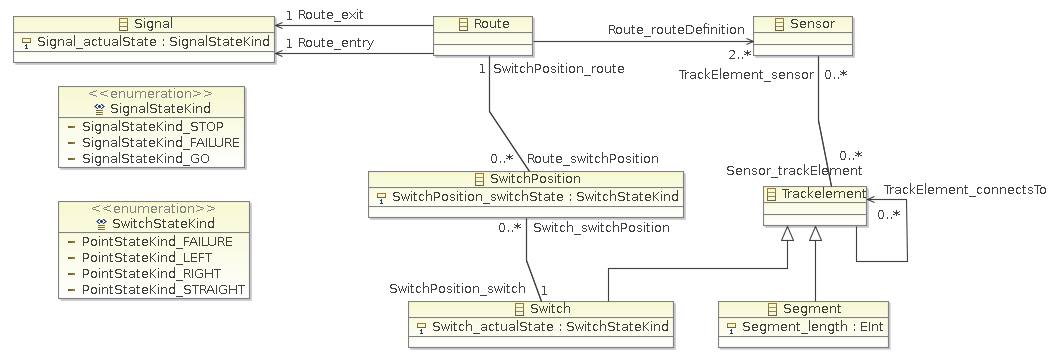
\includegraphics[]{figures/TrainMetamodel}
\caption{}
\label{fig:}
\end{center}
\end{figure}

